\documentclass[runningheads,a4paper]{llncs}

\usepackage{amssymb}
\setcounter{tocdepth}{3}
\usepackage{graphicx}

\usepackage{makeidx}  % allows for indexgeneration
\usepackage{amssymb, amsmath, amsfonts, graphics, graphicx}
\usepackage{enumerate}

\usepackage{longtable}

\usepackage{url}
\urldef{\mailsa}\path|{alfred.hofmann, ursula.barth, ingrid.haas, frank.holzwarth,|
\urldef{\mailsb}\path|anna.kramer, leonie.kunz, christine.reiss, nicole.sator,|
\urldef{\mailsc}\path|erika.siebert-cole, peter.strasser, lncs}@springer.com|
\newcommand{\keywords}[1]{\par\addvspace\baselineskip
\noindent\keywordname\enspace\ignorespaces#1}


%=======================================================================
%==========================DOCUMENT=====================================
%=======================================================================
\begin{document}

\newcommand{\fictAquantor}{\ensuremath{\forall\colon\boldsymbol{True}}}
\newcommand{\fictEquantor}{\ensuremath{\exists\colon\boldsymbol{True}}}
\newcommand{\bomega}{\boldsymbol{\omega}}
\newcommand{\bphi}{\boldsymbol{\phi}}
\newcommand{\eqdef}{\stackrel{\mathrm{df}}{=}}
\newcommand{\bigand}[2]{\raisebox{-4pt}{\ensuremath{\overset{#1}{\underset{#2}{\text{\huge\&\normalfont}}}}}}

\mainmatter  % start of an individual contribution

% first the title is needed
\title{Automated Theorem Proving Based on the Calculus of Positively Constructed Formulas\thanks{Ok}}
% a short form should be given in case it is too long for the running head
\titlerunning{ATP Based on the PCF Calculus}

% the name(s) of the author(s) follow(s) next
%
% NB: Chinese authors should write their first names(s) in front of
% their surnames. This ensures that the names appear correctly in
% the running heads and the author index.
%
\author{Alexander Larionov\and Artem Davydov\and Evgeny Cherkashin}
%
%\authorrunning{Lecture Notes in Computer Science: Authors' Instructions}
% (feature abused for this document to repeat the title also on left hand pages)

% the affiliations are given next; don't give your e-mail address
% unless you accept that it will be published
\institute{Irkutsk State University,
              1, Karl Marks str., Irkutsk, Russia \\
           Institute for System Dynamics and Control Theory at Siberian Branch
              of Russian Academy of Sciences,
              134, Lermontov str., Irkutsk, Russia\\
           Irkutsk National Research Technical University,
              83, Lermontov str., Irkutsk, Russia
%\mailsa\\
%\mailsb\\
%\mailsc\\
%\url{http://www.springer.com/lncs}
}

%
% NB: a more complex sample for affiliations and the mapping to the
% corresponding authors can be found in the file "llncs.dem"
% (search for the string "\mainmatter" where a contribution starts).
% "llncs.dem" accompanies the document class "llncs.cls".
%

\toctitle{Lecture Notes in Computer Science}
\tocauthor{Authors' Instructions}
\maketitle


%=======================================================================
%==========================ABSTRACT=====================================
%=======================================================================
\begin{abstract}
A description of the calculus of positively constructed formulas (PCF) and prover based on this calculus is considered in this paper. The PCF calculus has been developed by Russian scientists S.N. Vassiliev and A.K. Zherlov by an evolutionary way in describing and solving control theory problems. This calculus has features, which are applicable in control theory. The described implementation of the prover uses several techniques and strategies to improve prover performance. The prover is being tested by means of solving problems from TPTP library. The usage of implemented strategies is also commented in this paper.
\keywords{positively constructed formulas, automated theorem proving, proof strategies}
\end{abstract}



%=======================================================================
%==========================INTRODUCTION=================================
%=======================================================================
\section{Introduction}

Originally \cite{SNV1990,ICDS2000} the calculus of positively constructed formulas (PCF) was developed by Russian scientists S.N. Vassilyev and A.K. Zherlov by an evolutionary way in describing and solving control theory (CT) problems. In \cite{ICDS2000} the PCF calculus is presented as first-order logical formalism, examples of CT problems described  and solved by the PCF calculus (elevator group control, mobile robot action planning and telescope guidance), proof of soundness and completeness are presented as well.

The PCF calculus is positioned as not only machine-oriented, but also as a human-oriented, mostly aimed at solving the problems of dynamic systems control due to the following features of this calculus: unique inference rule and simple scheme of axioms; modifiability of semantics (constructive, monotonic, temporal, etc.) and besides it is possible to construct intuitionistic inferences of some non-Horn formulas; the explicit usage of $\forall$ and $\exists$ quantifiers, the scolemization procedure is not required.

However, in this paper, we will not cover the human--orientability properties of the PCF calculus and its dynamic systems control properties as well. We deal with the automatic search of a logical inference, as the inference engine capabilities are the basis of the problem solving systems, described in \cite{ICDS2000}. In order to estimate the applicability of the PCF calculus for automatic theorem proving we develop a prover program and test it on problems from TPTP library.

%This paper contains a description of the PCF calculus, an implementation of the prover program, and strategies of logical inference used to direct the inference search algorithms. The results of a comparison of the developed prover system with other provers are presented.


%=======================================================================
%==========================BACKGROUND===================================
%=======================================================================
\section{Background}
We consider the language of first-order logic consist in formulas build on atomic formulas with $\&, \vee, \neg, \rightarrow, \leftrightarrow$ operators, $\forall$ and $\exists$ quantifier symbols and constant operators $true$ and $false$. The terms term, atom, literal we define in the usual way. FOFs.

Let $X = \{x_1,\ldots,x_k\}$ be the set of variables, $A = \{A_1,\ldots,A_m\}$ be the set of atomic formulas, and $F = \{F_1,\ldots,F_n\}$ be the set of some FOFs. Then the following formulas $((\forall x_1) \ldots (\forall x_k) (A_1 \& \ldots \& A_m \rightarrow (F_1 \vee \ldots \vee F_n)))$ and $((\exists x_1) \ldots (\exists x_k) (A_1 \& \ldots \& A_m \& (F_1 \& \ldots \& F_n)))$ are denoted as  $\forall_XA\colon F$ and $\exists_XA\colon F$ respectively, keeping in mind that the $\forall$--quantifier corresponds to $\rightarrow F$, where $F$ means disjunction of all formulas from $F$, and $\exists$--quantifier corresponds to $\& F$, where $F$ means conjunctions of all formulas from $F$.

If $F = \emptyset$, then the formulas have the form $\forall_XA\colon\emptyset \equiv \forall_XA \rightarrow false$ and $\exists_XA\colon\emptyset \equiv \exists_XA \& true$, since the empty disjunction is identical to $false$, whereas the empty conjunction is identical to $true$. The form $\forall_XA$ and $\exists_XA$ are abbreviations of the [abovementioned] formulas. If $X = \emptyset$, then $\forall A\colon F$ and $\exists A\colon F$ are analogous abbreviations.

The set of atoms $A$ is called {\em conjunct}. The empty conjunct is identical to $true$ as it was already mentioned.

Variables from $X$ are bounded by correspoding quantifiers and called $\forall$--variables and $\exists$--variables, respectively. In $\forall_XA$ a variable from $X$ that does not appear in conjunct $A$ is called {\em unconfined} variable.

%В связи с изложенными сокращениями отметим следующий факт:
$\forall \emptyset \equiv \forall \emptyset\colon\emptyset \equiv \forall true \rightarrow false \equiv false$

Construction $\forall_XA$ and $\exists_XA$ are called positive typical quantifiers (TQ), because $A$ is a conjunction of only positive atoms meaned as typical condition for $X$. In practise, this constructions denote the following phrases: ``for all $X$ satisfying $A$ there is...'' or ``there exists $X$ satisfying property $A$ such that...''. For example, ``for all integer $x,y,z$ and $n>2$ there is $x^n + y^n \ne z^n$''.

Originally, the term ``typical quantifier'' was introduced by N. Bourbaki \cite{Bourbaki} as part of notation for formalisation of mathematics. But typical quantifiers are stable in the languages of another applied fields.

%========================================================
\section{The Method of PCF}

\subsection{PCF Language}

\begin{definition}[Positively--constructed formulas (PCF)]
\label{def:pcf}
Let, $X$ be the set of variables, and $A$ be a conjunct.
\begin{enumerate}

\item $\exists_XA$ and $\forall_XA$ are $\exists$--PCF and $\forall$--PCF respectively.

\item If $F = \{F_1,\ldots,F_n\}$ are $\forall$--PCF, then $\exists_XA\colon F$ is a $\exists$--PCF.

\item If $F = \{F_1,\ldots,F_n\}$ are $\exists$--PCF, then $\forall_XA\colon F$ is a $\forall$--PCF.

\item Any $\exists$--PCF or $\forall$--PCF is a PCF.
\end{enumerate}
\end{definition}

This form of logical formulas is referred to as positively constructed formulas (PCFs), as they are written with only positive type quantifiers. The formulas contain no explicit logic negation sign. Any FOF can be represented as PCF \cite{ICDS2000}.
%Таким образом ПО--формула есть особый вид записи классических формул языка предикатов, подобно КНФ, ДНФ и др.

PCF that started from $\forall \emptyset$ is called PCF in {\em canonical form}. Any PCF can be represented in the canonical form. Let $F$ is a $\exists$--PCF, then formula
$\forall \emptyset\colon F \equiv true \rightarrow F \equiv F$. If $F$ is a non-canonical $\forall$--PCF, then $\forall \emptyset\colon\{\exists \emptyset\colon F\} \equiv true \rightarrow \{true\&F\} \equiv F$. Typical quantifiers $\forall \emptyset$ and $\exists \emptyset$ are called {\em fictitious}, since they does not influence on truth of original PCF and does not bound any variables.  %а только лишь служат конструкциями сохраняющими корректную запись ПОФ.

%Для удобства читаемости формул, будем представлять их в древовидной форме следующим образом:
The PCFs are usually represented as a tree for more ease reading:
$$Q_XA\colon\{F_1,\ldots,F_n\} \equiv Q_XA \left\{
\begin{array}{lcl}
 F_1 \\
 \ldots \\
 F_n
\end{array}
\right.,$$

\noindent{} where $Q$ is a quantifier. The tree elements have conventional names: node, root, leaf, branch etc. As the quantifiers $\forall$ correspond to disjunctions of formulas $\{F_1,\ldots,F_n\}$, (quantifiers $\exists$ correspond to a conjunction), then, in a general case, all $\forall$-nodes correspond a {\em disjunctive branching}, and for $\exists$-nodes correspond to {\em conjunctive branching}.

Some parts of canonical PCF are named as follows:
\begin{enumerate}
\item PCF root $\forall \emptyset$ is called {\em PCF root};
\item PCF root children $\exists_XA$ are called {\em PCF bases}, conjunct $A$ is called {\em base of facts}, and PCF rooted from base is called {\em base subformula};
\item PCF bases children $\forall_YB$ are caled {\em questions} to parent base. If question is a leaf of tree then it is called {\em goal question}.
\item subtrees of questions are called {\em consequents}. The consequent of goal question is $false$.
\end{enumerate}

%как правило
In the sequel, only PCFs in the canonical form are considered.
%----------------------
%EXAMPLE
%----------------------

%ПО-формулы имеют древовидную структуру, а значит можно использовать соответствующую терминологию и изображать их как деревья.+++++++++++++++++++++++++
%PCFs have a tree-like structure, therefore we can use corresponding terminology and represent PCFs as trees.
%Any $\forall$--variable that does not occur in the corresponding conjunct is called {\em unconfined} variable.

Some parts of a PCF are denoted by particular terms: the topmost (0-depth) node is called {\em root}; a 1-depth node is called {\em base} (of formula); a maximal subtree that rooted at the 1-depth node is called {\em base subformula}; a 2-depth node is called {\em question} (to its base); a maximal subtree that rooted at the 2-depth node is called {\em question subformula}; a maximal subtree that rooted at 3-depth node is called {\em consequent} (subformula). With respect to Definition~\ref{def:semantic} if an even-depth (odd-depth) node has more than one children then the node has {\em disjunctive branching} (correspondingly {\em conjunctive branching}).%; if a node of PCF has a following form $\forall \bar{x}\colon A$ and if $\exists v \in \bar{x}$ and $v \notin A$ then variable $v$ is called {\em unconfined} variable. %The semantics of the denotation used results from the above mentioned human--orientation of the PCF calculi.

\begin{example}
Let us consider a formula of FOL.
$$F= \neg\bigl(\forall x\:\exists y P(x,y)\rightarrow \exists z P(z,z)\bigr).$$
An image $F^{\text{\tiny{PCF}}}$ of $F$ in the PCF language is

$$F^{\text{\tiny{PCF}}} = \forall\colon \boldsymbol{True}(\exists\colon\boldsymbol{True}(\forall x\colon\boldsymbol{True}(\exists y\colon P(x,y)), \forall z\colon P(z,z)(\exists\colon\boldsymbol{False}))).$$
%А эта ПО-формула в древовидной форме имеет следующий вид+++++++++++++++++++++++++
The tree--like form of the above PCF is as follows:
$$F^{\text{\tiny{PCF}}} = \forall\colon \boldsymbol{True}-\exists\colon\boldsymbol{True} \left\{
\begin{array}{lcl}
 \forall x\colon\boldsymbol{True} & - & \exists y\colon P(x,y) \\
 \forall z\colon P(z,z) & - & \exists\colon\boldsymbol{False}.
\end{array}
\right.$$
\end{example}
%Для удобствоа мы используем символ --- для обозначения рёбер в древовидном представлении ПО-формулы. Фугрная скобка также является вспомогательным символом.+++++++++++++++++++++++++
For convenience we use symbols ``--'' and ``\{'' for denoting the edges and branching in tree--like representation of PCF.

\subsection{Inference rule}

\begin{definition}[Answer]
\label{answer}
Let us assume that a question $\forall_YB:\Upsilon$ to a base $\exists_XA$ has an {\em answer} $\theta$ if and only if $\theta$ is a substitution $Y \rightarrow H^{\infty} \cup X$ and $B\theta \subseteq A$, where $H^{\infty}$ is Herbrand universe based on constans and function symbols that occur in corresponding base subformula.
\end{definition}

\begin{definition}[Splitting]
\label{splitting}
Let $F = \exists_XA\colon\Psi$, and $S = \forall_YB\colon\Upsilon$, where $\Upsilon = \{\exists_{Z_1}C_1\colon\Gamma_1,\ldots,\exists_{Z_n}C_n\colon\Gamma_n\}$ then $split(F,S) = \{\exists_{X \cup {Z_1}'} A \cup {C_1}'\colon\Psi \cup {\Gamma_1}',\ldots,\exists_{X \cup {Z_n}'} A \cup {C_n}'\colon\Psi \cup {\Gamma_n}'\}$, where $'$ is a variable renaming operator. We say that $F$ splitted by $S$. Obviously, $split(F,\forall_YB) = split(F,\forall_YB\colon\emptyset) = \emptyset$.
\end{definition}

\begin{definition}[$\omega$ inference rule]
Consider some canonical PCF $F = \forall\emptyset\colon\Phi$. Let there exists a question $Q$ that has an answer $\theta$ to appropriate base $S \in \Phi$, then $\omega F  = \forall \emptyset\colon\Phi \setminus \{S\} \cup split(S,Q\theta)$.
\end{definition}

In other words, if a question has an answer to its base, then the base subformula is splitting by this question. In the case of the goal question, we say that the basic subformula is refuted because $split(S,\forall_YB) = \emptyset$. The refuted base subformula $S$ removed from the set of base subformulas $\Phi$, since $\Phi \setminus \{S\} \cup \emptyset = \Phi \setminus \{S\}$

Once refuted all bases subformulas from $\Phi$, the formula $F$ is also refuted, since $\forall \emptyset\colon\emptyset \equiv false$. %согласно правилу описанному выше

%Note that the answer the questin with the disjunctive branching leads to an increase

%Отметим, что ответ на вопрос с дизъюнктивным ветвлением приводит к увеличению количества базовых подформул в силу использования оператора расщепления, а опровержение базы уменьшает количество баз на одну опровергнутую.

%----------------------
%EXAMPLE
%----------------------
\begin{example}[A refutation in $\boldsymbol{JF}$]\label{proofexample}


\begin{equation*}\label{ex:f1}
  F_1 = \forall\colon\boldsymbol{True} - \exists\colon S(e)(Q_1,Q_2,Q_3,Q_4);
\end{equation*}
\begin{equation*}
  \begin{array}{l}
  Q_1 = \forall x\colon S(x) - \exists\colon A(a); \\
  Q_2 = \forall x,y\colon C(x),D(y) - \exists\colon\boldsymbol{False}; \\
  Q_3 = \forall x,y\colon B(x),C(f(y)) - \exists\colon\boldsymbol{False}; \\
  Q_4 =
  \forall x\colon A(x) -
  \left\lbrace
  \begin{array}{l}
    \exists y\colon B(y),C(f(x)) \\
    \exists \colon C(x) - \forall z\colon A(z),C(z) - \exists\colon D(f(z)).
  \end{array}\right.
  \end{array}
\end{equation*}
At the first step only one answer $\{x \rightarrow e\}$ to question $Q_1$ exists. After applying rule $\bomega$ with this answer, formula will be in the following form:
\begin{equation*}\label{ex:f2}
  F_2 = \forall\colon\boldsymbol{True} - \exists\colon S(e),A(a)(Q_1,Q_2,Q_3,Q_4).
\end{equation*}
At the second step also only one answer $\{x \rightarrow a\}$ to  question $Q_4$ exists. After applying $\bomega$ with this answer, formula is split, because $Q_4$ has disjunctive branching. And now formula has the following form:

\begin{equation*}\label{ex:f3}
F_3 =
\forall:\boldsymbol{True} -
\left\lbrace
\begin{array}{l}
  \exists y_1\colon S(e),A(a),B(y_1),C(f(a)) -
  \left\lbrace
  \begin{array}{l}
    Q_1 \\ \cdots \\ Q_4
  \end{array}\right. \\
  \exists\colon S(e)A(a),C(a) -
  \left\lbrace
  \begin{array}{l}
    Q_1 \\ \cdots \\ Q_4 \\
    \forall z\colon A(z),C(z) - \exists\colon D(f(z)).
  \end{array}\right. \\
\end{array}\right.
\end{equation*}

At the third step first base can be refuted by answering on $Q_3$ goal question with $\{x \rightarrow y_1; y \rightarrow a\}$. Refuted base (base subformula) can be deleted from the list of base subformulas.

At the fourth step the answer $\{z \rightarrow a\}$ to fifth new question exists. And now formula has the following form:
\begin{equation*}\label{ex:f5}
  F_4 = \forall\colon\boldsymbol{True} - \exists\colon S(e),A(a), C(a),D(f(a))
  \left\lbrace
  \begin{array}{l}
    Q_1 \\ \cdots \\ Q_4 \\
    \forall z\colon A(z),C(z) - \exists\colon D(f(z)).
  \end{array}\right.
\end{equation*}

At the fifth step the only base can be refuted by answering on $Q_4$ goal question with  answer $\{x \rightarrow a; y \rightarrow f(a)\}$.

The refutation is finished because all bases were refuted.

\end{example}


%=======================================================================
%==========================TECHNICQUES==================================
%=======================================================================
\section{Prover implementation}

\subsection{Implementation language}

Our prover is implemented in the D programming language \cite{DPL1,DPL2}. The D programming language has many features: compiler produce a native binary code, which both fast and optimized; procedures of memory management are manually adjustable, but it is also possible to use garbage collection; there is a good library for parallel computation construction in Erlang--like model, which is generally recognized as the quite good \cite{Erlang1}.

\subsection{Proof State Tree}

%---------
%One of the basic components of our prover implementation is a proof states tree (PST).

Each step of the inference in the PCF calculus can be considered as an addition of corresponding consequent subformulas to the base subformula (facts to a base; questions to a question lists). Thus, a formula is usually monotonically increasing, and splitting if a disjunctive branching happens.
%---------

One of the main tools of the logical inference search implementation in the developed prover is the \emph{proof state tree} (PST), which is built with the data structures based on so--called chunks described below. The PST structures are used to store the sequence of the steps of logical inference. Each step corresponds to a single operation that were performed. PST also represents the current state of the formula under refutation. The main purpose of PST is to strictly fix all operations and their parameters, which occurs on every step of logical inference construction. The example of such operation is the fact of applying a substitution in a base subformula to a question.

%--------------------------------------------------------------------------------
\subsubsection{Chunk.}
Chunk is a single--linked list of elements with type {\tt T} which have not only reference to the \texttt{first} and \texttt{last} elements of that list. A chunk is empty, if it does not contain any elements, and \texttt{first} and \texttt{last} elements are NULL--references. We say, that chunk $C_1$ is \emph{linked} with chunk $C_2$ \emph {from the left}, if the \texttt{last} node of chunk $C_1$ is referring to the \texttt{first} node of chunk $C_2$ and, simultaneously, $C_2$ linked with $C_1$ \emph{from the right}. For this operation a procedure of linking {\tt void link(Chunk!(T) c)} is defined, which links current chunk and chunk {\tt c} from left. If the chunks are not empty, then linking is proceeded according to the definition. If one of the chunks is empty, then its \texttt{first} and \texttt{last} elements will be assigned to the value of the linking element. Note, that several chunks can be linked with different chunk from one of its sides simultaneously. Therefore, using the procedure of linking one can build a tree of chunks, which grows from leafs.

%With the chunks we can organize main storage of information of PCF and the states of logical inference.

In Fig.~\ref{fig:chunk1} an example of structure is presented, which is built from chunks.
\begin{figure}[h]
  \vspace{0.5cm}
  \centering
  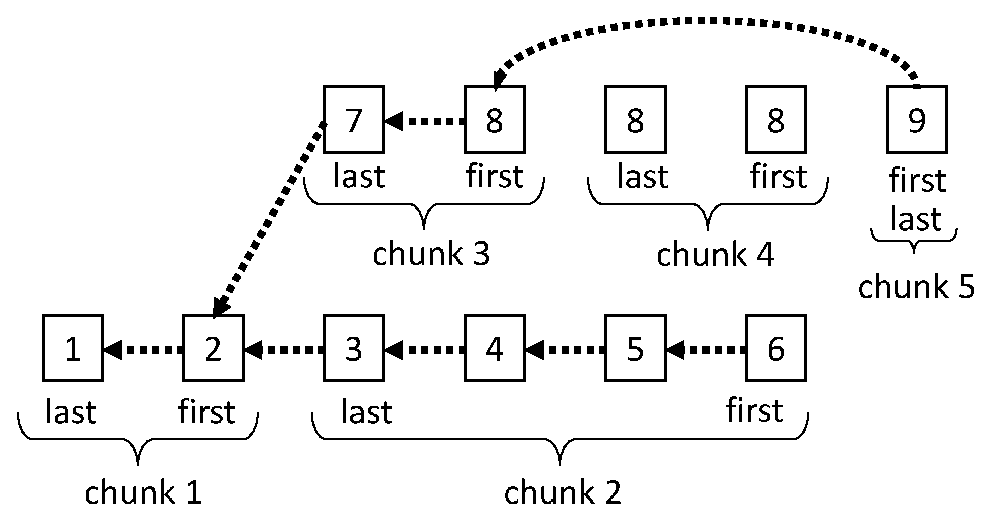
\includegraphics[width=0.6\linewidth]{img/ChunkFullp1.eps}
  \caption{Chunks}
  \label{fig:chunk1}
\end{figure}
There are five chunks in this figure, and several of them are linked together with \texttt{first} field: ``5'' and ``4'', ``4'' and ``3'', ``3'' and ``1'', ``2'' and ``1''. Chunk 4 is empty. \texttt{first} and \texttt{last} is the first and last nodes of chunks. Numbers are the identifiers of the corresponding nodes. Empty chunk duplicates node \texttt{first} for the node linked with empty chunk from the left.


%---------------------
\subsubsection{Proof state tree.}
A proof state tree is a tree with the following properties: the root is the original PCF, other nodes are consequent subformulas (with the answer applied to them and variables renamed). In addition, the nodes contain some system information like step of inference, answer, etc. Thus, the number of the leafs is the current number of the bases, and at current inference step a PCF is denoted by the path from the leaf to the PST root. This approach allows us to rollback (backtrack) the inference search process, observe proof states and share references among terms and formulas. If a base is refuted then its memory can be released by deleting of the path from corresponding leaf to the soonest branching.

Every node of PST is a chunk. The growth of the tree is a linking of new chunks with the existing leafs of the tree from the left.

PST for the formula from Example \ref{proofexample} is represented in Fig.~\ref{fig:pst}.
PST root is an original PCF $F_1$. Node ``2'' is a  $Q_1$ question consequent $\exists\colon A(a)$, and the path from node ``2'' to the root node corresponds to PCF $F_2$. Nodes ``3'' and ``4'' are corresponding consequents for $Q_4$. The path from node ``3'' to the root node and the path from node ``4'' to the root node correspond to base subformulas for PCF $F_3$. For example, formulas that are denoted by paths ``5''--``1'' and ``3''--``1'' share data that are represented by nodes ``1''--``2''. When base subformula that is represented by path ``3''--``1'' is refuted, we can delete path from node ``3'' to soonest branching --- in this case only node ``3'' is deleted, because nodes ``2''--``1'' are still used for representing another base subformulas.
%The lettering in figures should have a height of 2mm (10-point type)
%caption UNDER the figures
\begin{figure}[h]
  %\vspace{0.5cm}
  \centering
  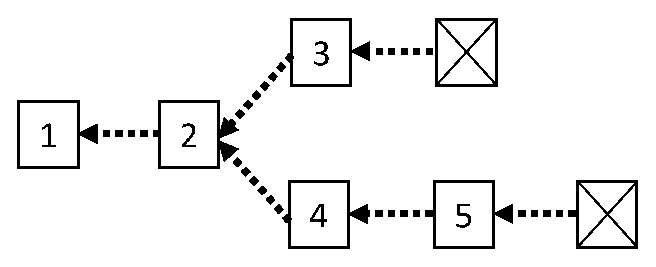
\includegraphics[width=0.4\linewidth]{img/PSTp1.eps}
  \caption{Proof state tree for PCF from Example \ref{proofexample}.}
  \label{fig:pst}
\end{figure}

%---------------------
\subsubsection{Data sharing: sharing of base subformulas.}
%------
In addition, in a PST the data--sharing (memory sharing) is implemented: if two base subformulas are characterized by the corresponding paths, their bases share data, which are represented by the same part of these paths.
\begin{figure}[h]
  \vspace{0.5cm}
  \centering
  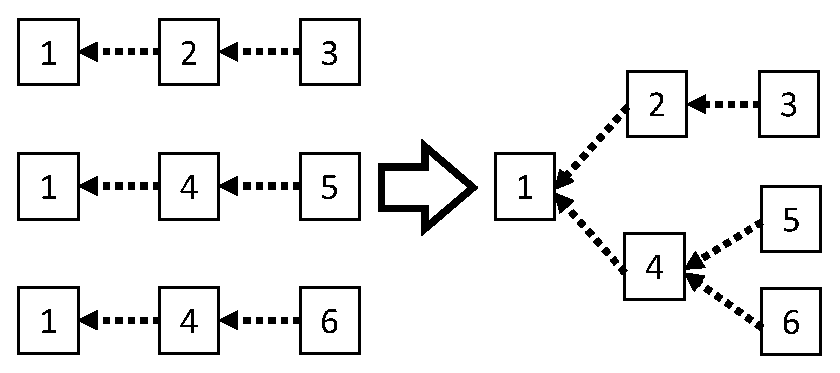
\includegraphics[width=0.4\linewidth]{img/Graphsp1.eps}
  \caption{Example of proof state tree for base subformula refutation}
  \label{fig:datasharing1}
\end{figure}

If a PCF contains a question with disjunctive branching, then its base subformula will be divided into several new base subformulas during the searching procedure of the logical inference. The number of new subformulas corresponds to the number of disjunctive subformulas in the consequent of the question. In the straightforward variant of the prover implementation, the sharing will require copying previous state of the original formula more than once; this copying have a linear complexity, but it leads to the redundant expenses of memory and processor time. PST allows one to implement sharing the common subbranches. Let's we have the following base subformula:
$$\exists: A(a) - \forall x: A(x) - \left\{
\begin{array}{lcl}
 \exists \colon B(x) & - & \forall y: B(y) - \exists\colon\boldsymbol{False}\\
 \exists \colon C(x) & - & \forall y: C(y) - \exists\colon\boldsymbol{False}
\end{array}
\right. $$

Note, that the formula has disjunctive branching and it is deep. PST for the refutation of this base subformula is presented on Fig.~\ref{fig:datasharing2}
\begin{figure}[h]
  \vspace{0.5cm}
  \centering
  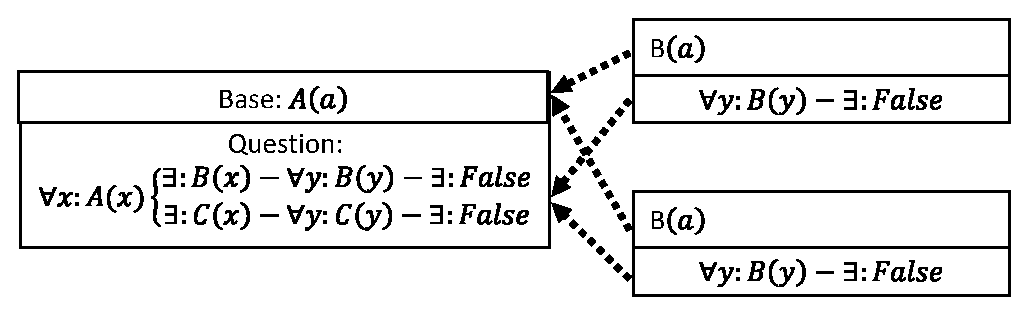
\includegraphics[width=0.82\linewidth]{img/DataSharing2p1.eps}
  \caption{Example of proof state tree for base subformula refutation}
  \label{fig:datasharing2}
\end{figure}




%====================================================================================
%====================================================================================
\subsection{Lazy concretization}

By the Definition~3 the inference rule $\omega$ can be applied if the question $\forall \bar{y}\colon A$ to base $\exists \bar{x}\colon B$ has an answer $\theta$, such that $\theta$ is a substitution $\bar{y} \rightarrow H^{\infty}$ and $A\theta \subseteq B$. If all the variables in the $\bar{y}$ are occurred in $A$, then the search of corresponding elements from $H^{\infty}$ is carried on by the algorithm of subsumption and depends on only corresponding base of facts, hence the conditions of sets subsumptions need to be satisfied. If a variable in the $\bar{y}$ is not occurred in $A$ then the variable is called {\emph unconfined variable} and it is not used in a subsumption. However, we need to find a substitution for these variables as well, and any element of Herbrand universum is a correct substitution. The problem with Herbrand universum is that in the general case, it is an unlimited set and it is not known what element should be taken as a substitution.

The main concept of lazy concretization is as follows. Instead of selection of a concrete element of the Herbrand universum for a substitution of an unconfined variable an {\em unspecified Herbrand element} (UHE) is used temporally. The UHE will be concretized further to a proper term. Such concretization is based on the logical inference requirements. UHE will be concretized to a ground term, or in some situations, it will remain unconcretized. In such case, the required terms provide the possibility of answering to the question: UHE is gradually concretized in such way, that on every step of inference we can build new answer for some question. Simultaneously the following problem is being solved: to what term we need to concretize UHE to make it possible to answer the question? Note, that originally UHE appears as a part of answer in one question and its concretization is done while searching the answers for other questions. As ``gradually concretization'' we mean procedure of lazy computations: UHE concretized as precise, as it is enough for answering the current question, i.e. concretization, generally, is partial, for example UHE for $h$ is concretized to $f(h_1)$, where $h_1$ is a new UHE.

By it's nature UHE is similar to unconcretized $\forall$-variable in the sense that it is mutable, i.e. it is potentially concretized, however all such changes must be directed only to concretization of UHE, i.e. UHE is substituted only to some term or to different UHE, but not to the variable.

Let's consider the example of this technique in process of building the logical inference for the following formula.
\begin{equation*}
  \forall\colon\boldsymbol{True} - \exists\colon\boldsymbol{True} -
  \left\lbrace
  \begin{array}{l}
    \forall x\colon\boldsymbol{True} - \exists\colon A(x) \\
    \forall x\colon A(f(x)) - \exists\colon B(f(x)) \\
    \forall\colon B(f(a)) - \exists\colon \boldsymbol{False}
  \end{array}\right.
\end{equation*}

At the first step an answer $\{x \rightarrow h_1\}$ to the first question exists, $x$ is an unconfined variable and $h_1$ is an unspecified Herbrand element. After this step the atom $A(h_1)$ is added to the base. At the second step an answer $\{x \rightarrow h_2\}$ to the second question exists and $h_1$ is concretized to $f(h_2)$, after this step $B(f(h_2))$ is added to the base. Finally, at the third step the trivial (empty) answer exists to the third question and $h_2$ is concretized to $a$.

For efficiency increase in this strategy, we are using two constraints.

%Для стртегии ленивой конкретизации предложено два типа ограничений
\subsubsection{Constraint~1: Limit of concretizations number.}
%Ограничение количества конкретизаций.

%---
Two UHEs are \emph{similar}, if they appear as the result of a substitution for the same unconfined variable. This situation appears if for a question with unconfined variables a sequence of answers were constructed, such that on every step of the sequence new UHE created as a substitution. A constraint for the similar UHE--concretizations excludes such situations, when UHE is concretized on a step, where it is not necessary, and, consequently, an opportunity to concretize it appears on other step. For every UHE a reference to the unconfined variable is stored, which the UHE was selected as a substitution for. The set of terms, which concretized a unconfined variable through its UHE, is stored in the corresponding question. The engine allows tracking the UHE concretization. If a predefined limit of the concretizations is exceeded then all further concretizations are denied. The limit is chosen by user using additional information about the problem under investigation, or it is taken as $1$, and increased after an unsuccessfull logical inference, then the inference attempt is repeated.

\subsubsection{Constraint~2: Storing expressions which contain UHE.}
%Сохранение выражений, содержащих НЭЭ

For a question with unconfined variables, one can apply all available answers, i.e. with using all elements of Herbrand universum. It is known, that this is not technically possible because of unlimited Herbrand universum. So, the technique of lazy computations is used. In ideal case, all answers for question is used simultaneously, but actually only the required questions are used. For example, if in a some formula $\forall x: True  - \exists A(x)$, and $H^{\infty}= \{a, f(a), f(f(a)), ...\}$ then usage of all available questions simultaneously leads to addition of $\{A(a), A(f(a)), A(f(f(a))), ...\}$ elements (amount is unlimited) to the base. Instead, this set is associated with the element $A(h)$, where $h$ is UHE, and this element generate required elements of $H^{\infty}$ set in further.

In such case, one can find a similarity with lazy concretization strategy without constraints. The advantage of the approach with storing expressions, which contain UHE, is that the expression with UHE is always stored, i.e. it is not possible to lose it by applying some substitutions.


%====================================================================================
%-----------------k,m,-condition-----------------
\subsection{Strategy ``k,m-condition"}
An answer to a question is accepted if at some point of the following $k$ steps of its inference a certain condition becomes true at least $m$ times. This strategy is used in the following cases.

\subsubsection{$k,m$--refutation.} An answer to a question with disjunctive branching is accepted if in next $k$ steps at least $m$ generated bases were refuted, otherwise the process restarted with a new answer. This strategy allows us to constrain highly spawning inferences by means of control answering questions with disjunctive branching.

\subsubsection{$k$--unrefutation.}
For a question with disjunctive branching an answer is accepted if during next $k$ steps no refutation for the base subformula was achieved, using the questions without disjunctive branching. This strategy, as it is in the previous variant, reduces growth of a formula due to answering questions with disjunctive branching. If no refutation can be constructed using this strategy, then answering to the questions allowed. The parameter $m$ is dropped in that case.

\subsubsection{$k,m$--concretization.}
An answer for a question is accepted if during next $k$ steps at least $m$ UHE are concretized. This strategy is also aimed at limiting a complexity of the formula. Large amounts of additional information and conditions are associated with unconcretized UHE. After an UHE is concretized, the associations are released. So as soon we process the UHE as soon we will take advantage of additional memory.


%====================================================================================
%Parallel strategy
\subsection{Parallel strategy}

Let's consider techniques and strategies for parallel implementations of logical inference algorithms in the PCF calculus.

\subsubsection{First parallel strategy.}
If a question has disjunctive branching then, after we have answered that question, the formula will splits and transforms to the formula with number of bases equals to the number of answered question consequents, i.e. in general case the number of the base subformulas is increasing on every step of logical inference. In addition, the original formalization of a problem in PCF language can contain more than one base subformula. In order to refute the original PCF formula every base need to be refuted. The refutation of the base subformulas can be processed in parallel, i.e., the refutation of each base is processed in an independent thread. This is possible if the bases are independent from each other, i.e. they don't share $\forall$--variables and UHEs. Bases never share $\forall$--variables because bases don't contain $\forall$--variables at all (by definitions), as they contain only ground terms. However, bases can share the UHEs in case of usage of the lazy concretization strategy. Therefore, this strategy can be applied in case if the lazy concretization strategy is not used. According to the above described features of PCF we say, that PCF have property called ``OR--parallelism''.

\subsubsection{Second parallel strategy.}
In addition to the OR--parallelism, parallel schemes of algorithms for searching answers for each questions can be constructed. Since the questions do not share variables, as in previous strategy, the answer search procedure can be performed also in an individual computation thread. In addition, like in the previous strategy, second parallel strategy formulated as follows: each answer search procedure to a question is independent of other questions.

\subsubsection{Recomendation.}
One recommendation for an implementation of the described algorithms on cluster computing systems can be given: there is a problem to divide tasks between computing nodes depending on connection speed between the nodes. For example, implementation of the first strategy must bind process to the computing node. Binding the process to the computing node in case of second strategy is possible with increasing the conjunct of question and increasing the set of substitutions corresponding to the every atom of question. Otherwise, communication expenses can override the time of computation and will degrade the overall result.

\subsection{Memory manager}
Allocation of memory for fixed size records is implemented based on standard approach, which is similar to \cite{gmemory}. Array of structures is allocated with memory manager of operation system and then converted to freelists. New structures are allocated from the freelists, and released ones are returned back to the freelists. If a list is exhausted a new array is allocated from heap memory.

In the prover for each variant of records, own array is allocated and own freelist constructed. The garbage collection is synchronized with garbage collector of the D programming language runtime engine.


%=======================================================================
%==========================EXPERIMENTS==================================
%=======================================================================
\section{Experiments}
Testing the developed prover was performed on problems form TPTP \cite{tptp} library version 5.4.0 (Thousands of Problems for Theorem Provers, www.tptp.org). This library is the de facto standard for testing the ATP provers. The type of problems that were chosen are the problems of FOF without equality. Total number of problems is 1221 with rating from 0.0 to 1.0. Total number of solved problems is 780. The maximal rating of solved problem is 0.62. The best results among domains presented in the Table~1.

\begin{table}
\caption{Domains}
\begin{tabular}{|p{0.3\linewidth}|p{0.4\linewidth}|p{0.1\linewidth}|}

\hline
\textbf{Domain} & \textbf{No of problems in the domain} & \textbf{Solved} \\
\hline
Geometry (GEO) & 242 & 204 \\
\hline
Management (MGT) & 22 & 22 \\
\hline
Syntactic  (SYN) & 275 & 180 \\
\hline
Semantic Web  (SWB) & 25 & 22 \\
\hline
\end{tabular}
\end{table}

10 hardest problems solved by our prover is presented in the Table~2.
\begin{table}
\caption{Hardest problems solved by our prover}
\begin{tabular}{|p{0.2\linewidth}|p{0.2\linewidth}|p{0.2\linewidth}|p{0.2\linewidth}|}

\hline
\textbf{Problem} & \textbf{Rating} & \textbf{Time (s)} & \textbf{Steps number} \\
\hline
COM008+1 & 0.62 & 1.9 & 33551 \\
\hline
LCL640+1.005 &  0.62 &  0.06 &  821 \\
\hline
LCL656+1.010 &  0.58 &  1.5 &  43 \\
\hline
SWB012+3 &  0.54 &  65.64 &  102428 \\
\hline
SYN353+1 &  0.54 &  0.002 &  33 \\
\hline
SYN548+1 &  0.54 &  0.01 &  15 \\
\hline
SWB020+2 &  0.5 &  0.6 &  618 \\
\hline
LCL666+1.005 &  0.5 &  0.35 &  2592 \\
\hline
KRS235+1 & 0.46 & 5.4 & 24406 \\
\hline
SWB029+3 &  0.38 &  55.27 &  98471 \\
\hline
\end{tabular}
\end{table}

%График...

Prover shown good results for problems, whose formalization in the PCF language contains quite large conjuncts.

\subsection{Translation from TPTP to PCF}
TPTP contains an axiom library, which consists of different files. Formula to be investigated is collected from the files. The collection is performed with special utilities such as \texttt{tptp4X}. The collected subformulas are passed to a translator from TPTP representation to the input language of the prover. The translator is implemented with the \texttt{hotptp-yl-parser-verbose} \cite{TPTPTrans} utility that translates input TPTP--files to abstract syntax trees. Translation component of the utility is generated on the base of syntactic analysis of the current specification of TPTP. Therefore, in each case of the specification refinement, the utility can be automatically updated (recompiled). Using this approach, we are able to adopt our prover to the new input language specification.

The abstract syntax tree is passed to translation component that imports the tree, translates the predicate formula or CNF, performs some reduction of subformulas by applying a set of rules, converts the formulas into the PCF language, performs additional reduction of the PCFs, renames the quantifier variables, and, at the last step, outputs the conversion result as textual representation of the problem in the language of the prover.


\subsection{Example of Formula}
Problem SYN380+1.p from TPTP library in our prover input language has a following form:
\begin{quote}
\texttt{\raggedright\noindent
\{\\
~~e[][]~\{\\
~~~~a[W][big\_r(W,W)]~\{\\
~~~~~~e[][False]~\{\}\};\\
~~~~a[X,Y][]~\{\\
~~~~~~e[][big\_r(X,Y)]~\{\};\\
~~~~~~e[Z][big\_q(Y,X)]~\{\\
~~~~~~~~a[][big\_q(Z,Z)]~\{\\
~~~~~~~~~~e[][False]~\{\}\}\}\}\}\\
\}\\
}
\end{quote}

\subsection{Example of solved problem}
Let us consider COM003+1.p (``The halting problem is undecidable'') problem with 0.33 rating.

The results of solving this problem by our prover and other provers are presented in Table~3.

\begin{table}
\caption{COM003+1.p solving}
\begin{tabular}{|p{0.2\linewidth}|p{0.35\linewidth}|}

\hline
\textbf{Prover} & \textbf{Time (s)} \\
\hline
Our prover & 0.05 \\
\hline
Vampire & 0.01 \\
\hline
iProver & 0.27 \\
\hline
leanCoP & 19.25 \\
\hline
EP & 54.45  \\
\hline
Zenon & 0.08 \\
\hline
\end{tabular}
\end{table}

%Рассмотрим задачу TPTP SYN548+1.

%В языке ПО-формул формализация выглядит следующим образом:

%Рейтинг 0.54. Время решения: 5.8с. Количество шагов: 82764.

%При решении данной задачи использовались стратегии: ленивая конкретизация (ограничение 1), $8$--неопровержимость, $8,1$--конкретизация, разделение данных по базе, агрессивное разделение термов.

%Let's consider problem SYN548+1 from TPTP.
%In PCF language formalization looks like the following:

%Rating is 0.54. Time for solving 5.8s. Number of steps: 82764.

%The lazy concretization (first constraint), $8$--unrefutation, $8,1$--concretization, data sharing in bases.



%==========================================================
\subsection{Comments on strategies}

%=============================
\subsubsection{Lazy concretization.}
Lazy concretization strategy allows one in most cases to find a substitution for an unconfined variable in acceptable time as compared to the sequential enumeration of Herbrand universum. The constraints are the most valuable part of this strategy, which allow to decrease the number of steps of logical inference in comparison to the unconstrained strategy. The decrease of the number of steps leads to a decrease of the problem solving time. Application of the constraint~1 is the best way of the inference time reduction in the case when a formula has questions with disjunctive branching and the constraint~2 in case if the formula contains no questions without disjunctive branching.


%=============================
\subsubsection{$k,m$--condition.}
The efficiency of this strategy reveals in the problems with disjunctive branching. In all cases of acceptable application of this strategy and correctly chosen parameters, the noticeable improvement is achieved.
%===========================
\subsubsection{Parallel stratgies.}
The important quality of parallel schemes of algorithms is their scalability, i.e., the performance improvement respect to increase of the number of computational nodes (CNs). That’s why the main characteristic of the prover productivity is not the time of execution of the program, but the ratio of program execution time in parallel mode on a given number of CNs to the program execution time on a single CN. The ratio is accounted for various number of CNs.

Experiments were carried out on the logical problems which PCF--formalizations have necessary properties for the parallel strategies: disjunctive branching, large number of questions, large conjuncts in questions. In Fig.~\ref{fig:parallel} the results of experiments are shown.

\begin{figure}[h]
  %\vspace{0.5cm}
  \centering
  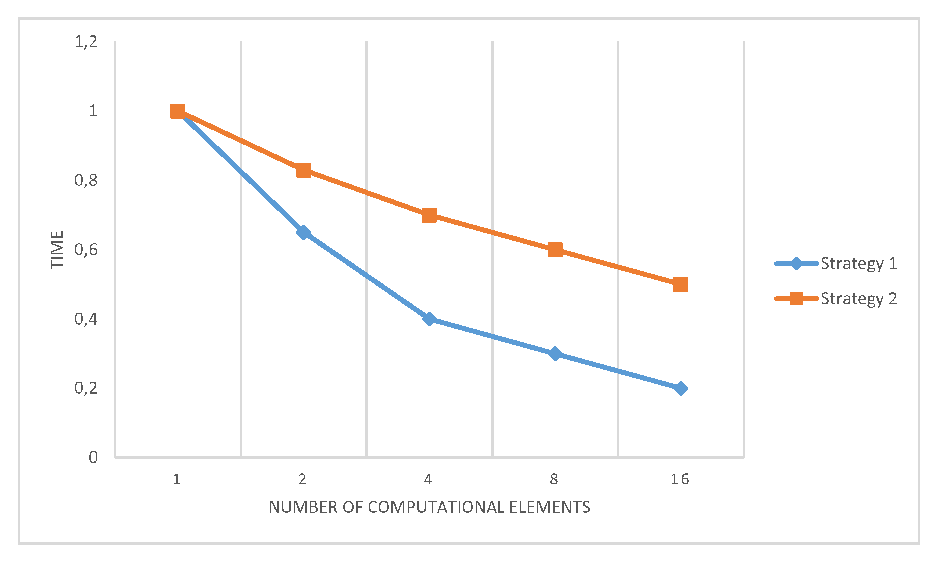
\includegraphics[width=0.8\linewidth]{img/Parallel.eps}
  \caption{Results of parallel strategies testing}
  \label{fig:parallel}
\end{figure}




%=======================================================================
%==========================CONCLUSION===================================
%=======================================================================
\section*{Conclusion}
In this paper, we presented the results of the PCF calculus investigation in the context of the automatic theorem proving. The main result is a prover program implemented based on the PCF calculus. Several logical inference strategies were devised, adopted from other papers and implemented in this prover: memory sharing, lazy concretization, $k,m$--condition, parallel strategies. A special global data structure (Proof state tree) has been developed. Most of the strategies are implemented on the base of the structure.

Testing our prover has been carried out on problems from TPTP library. Testing has shown that the PCF calculus is suitable for automated theorem proving and some problems are solved more efficiently than other provers. The classes of problems, which are the most suitable for our system, are described.

Further investigations aimed at implementation of a productive logical inference engine with equality and with indexing techniques, for example, substitution tree indexing \cite{subtree}. The application of this prover for solving the problems of dynamic systems control will be investigated also.



%=======================================================================
%==========================BIBLIOGRAPHY=================================
%=======================================================================
\begin{thebibliography}{4}

\bibitem{DPL2} Alexandrescu, A. The D Programming Language. -- Addison-Wesley Professional, 2010. -- 460p.

\bibitem{DPL1} Armstrong, J. D Programming Language. URL: http://www.digitalmars.com/d/.

\bibitem{Erlang1} Armstrong, J. Programming Erlang.  -- The Pragmatic Programmers, 2007. -- 519p.

\bibitem{TPTPTrans} Gelder, A.V. TPTPparser utility. 2006. URL: http://users.soe.ucsc.edu/\~{}avg/TPTPparser/.

\bibitem{gmemory} GLIB: Memory Slices. URL: http://developer.gnome.org/glib/2.34/glib-Memory-Slices.html.

\bibitem{subtree} Graf, P. Substitution Tree Indexing // Proceedings of the 6th International Conference on Rewriting Techniques and Applications. 1995. pp.~117--131.

%\bibitem{HAR} Robinson, A., Voronkov, A. (eds.) Handbook of Automated Reasoning. -- MIT Press, Cambridge, 2001. -- 2150p.

\bibitem{tptp} Sutcliffe, G. The TPTP Problem Library and Associated Infrastructure: The FOF and CNF Parts, v3.5.0 // Journal of Automated Reasoning. V43, N4, pp.337--362.

\bibitem{SNV1990} Vassilyev, S.N.: Machine Synthesis of Mathematical Theorems. The Journal of Logic programming, V.9, No.2--3, pp. 235--266 (1990)

\bibitem{ICDS2000} Vassilyev, S.N., Zherlov, A.K., Fedunov, E.A.,
Fedosov, B.E.: Intelligent Control of Dynamic Systems. Moscow: Fizmatlit (2000)(in Russian)

\end{thebibliography}




\end{document}

%%% Local Variables:
%%% mode: latex
%%% TeX-master: t
%%% End:
